\documentclass{article}
\usepackage{fancyhdr}
\usepackage{amsmath,amssymb}
\usepackage{geometry}
\usepackage{datetime}
\usepackage{enumerate}
\usepackage{graphicx}

%Insert page formatting here
%\hoffset = -.5in
\voffset = -0.375in
%\textwidth = 6in
\textheight = 8in
\headheight = 24pt

\pagestyle{fancy}

\rhead{Peter Olson\\Student ID: $441666$}
\lhead{Math 3200\\Homework 5}
\chead{\today}
\cfoot{}

%\addtolength{\headwidth}{\marginparsep}
%\addtolength{\headwidth}{\marginparwidth}

%\renewcommand{\labelitemi}{$\diamond$}
\renewcommand{\implies}{\rightarrow}
\newcommand{\widespace}{\qquad \qquad \;}
\newcommand{\tret}{\\ \hline}
\newcommand{\fh}{\tfrac{1}{2}}
\newcommand{\deriv}[2]{\frac{d #1}{d #2}}
\newcommand{\pderiv}[2]{\frac{\delta #1}{\delta #2}}
\newcommand{\vr}{\vec{r}}
\newcommand{\at}{\text{ at }}
\newcommand{\var}{\text{Var}}

\begin{document}
\section*{Exercise 5.28 + (c)}
	The resulting quantiles are very close to the Student-T distribution of $t_{4}$. $t_4$ has:
	
	
	25th Percentile: -0.7407
	
	50th Percentile: 0.0000
	
	90th Percentile: 1.533
	\\
	
	Furthermore, the histogram of $T^2$ appears to fit the distribution of $F_{1,4}$ quite well, with the granularity that I've specified. If I were just running a \texttt{plot(density(T$^2$))} on the data, then I would expect the curves to match up much better.
	\section*{Console Output}
	\begin{verbatim}
	> show(quantile(T, c(.25, .5, .9)))
	25%         50%         90% 
	-0.77883884 -0.04498658  1.31926928 
	\end{verbatim}
	\section*{R Code}
	\begin{verbatim}
	Z_vector <- vector()
	U_vector <- vector()
	
	for(i in 1:100){
	Z_vector <- c(Z_vector, rnorm(1, 0, 1))
	U_vector <- c(U_vector, rchisq(1, 4))
	}
	
	T <- 2 * Z_vector / sqrt(U_vector)
	
	show(quantile(T, c(.25, .5, .9)))
	
	plot(density(T))
	
	hist(T^2, freq=F, breaks = 30)
	#plot(density(T^2))
	curve(df(x,1,4), add=TRUE, lty = 2)
	\end{verbatim}
	\section*{Plots}
	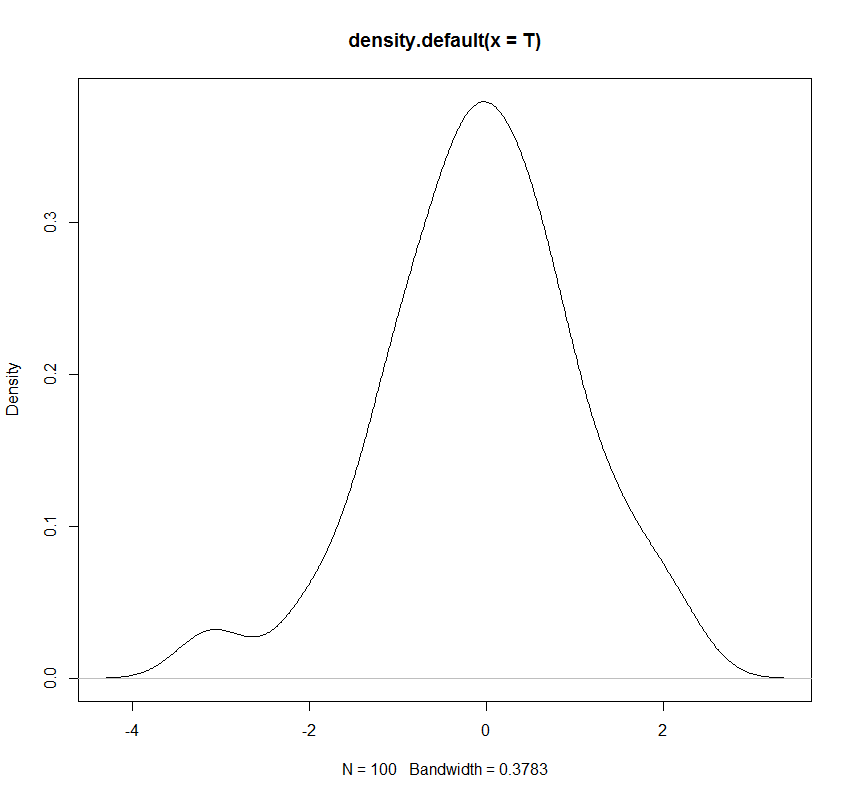
\includegraphics[width=4in]{q5}
	
	
	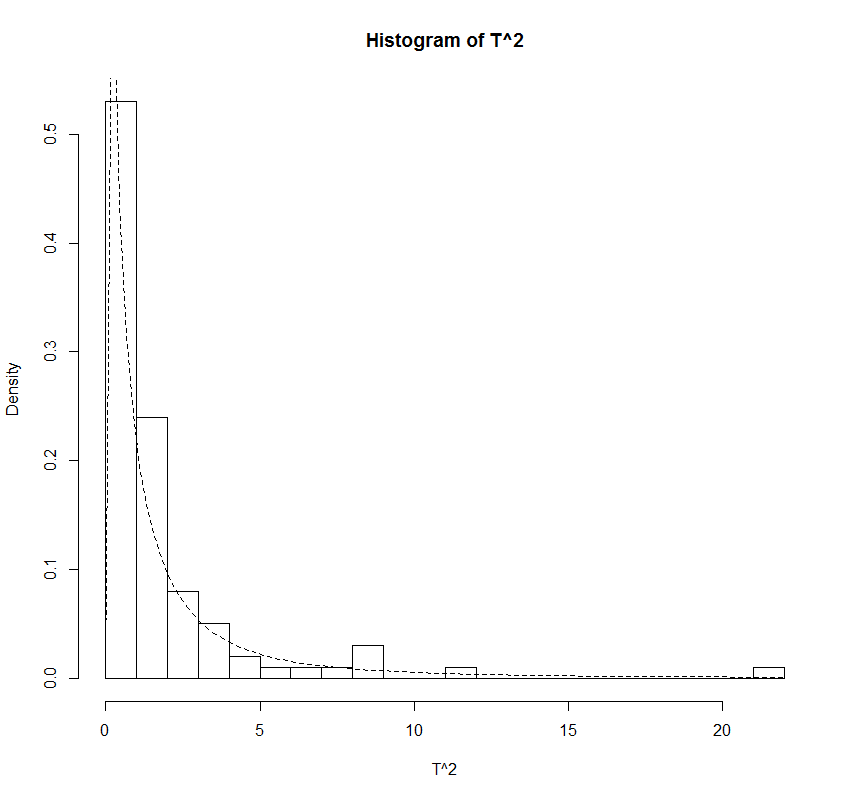
\includegraphics[width=4in]{q52}
\end{document}